\chapter{Numerically solving the scalar field collapse}

While studying gravitational collapse of a scalar field we got a set of differential equations. These differential equations were complicated enough that any effort to find an analytical solution was futile. One can always make approximations and get some understanding of the solutions, but to get the complete solution we need to use numerical techniques. In this chapter we will discuss about how to solve differential equations on a computer.




\section{Finite difference methods}

Solving differential equations is required in almost every field of Science and although analytical solutions are the best thing one can get, they are hard to get for any but the simplest systems.
Most of the time we have to resort to solving differential equation numerically. There a lot of methods out there developed to solve differential equations, each one of them have their own advantages and dis-advantages. In our case we will be using a class of methods called finite difference methods.

\index{Finite difference methods} Finite difference methods are among the most intuitive and easy to implement methods of solving differential equations. They are derived using the taylor series and give a discrete approximation of the strong from of a differential equation.

To get some intuition about finite difference methods let us start with a very simple example. These simple examples will demonstrate some of the most important concepts of finite difference computing.

Suppose that we want to find the derivative of $f(x) = x^3$ at $x =1$. We know that the answer should be $3$. But, let us say that we do not know the exact answer and want to approximate the derivative.
The simplest way to do this would be using the definition of differentiation,

\begin{equation}
    \frac{dy(x_0)}{dx} = \lim_{h \to 0}\frac{y(x_0 + h) - y(x_0)}{h}
\end{equation}

The definition gives us the exact answer in the limit $h \to 0$. What we can do is to take $h$ to be a small non-zero number and see if that gives us a good enough approximation.

\begin{equation}
    \frac{dy(x_0)}{dx} \approx \frac{y(x_0 + h) - y(x_0)}{h} , \text{for } h \ll 1
    \label{eq:first_order}
\end{equation}

We have shown the results of using the equation \ref{eq:first_order} to approximate the derivative of $x^3$ at $x=1$ in the figure \ref{fig:x^3_error_order1}. Y axis in the figure is the log error of the approximation and X axis is the log of the \index{step size} step size ($h$). Figure \ref{fig:x^3_error_order1} has a lot of stuff going on in it and we will break it down into parts. But, before we do that we will briefly look at how computers store decimal numbers and how does it affect our calculations.

\subsection{Floating point arithmetic}

\index{Floats} Floats are how computers internally represent decimal numbers. A larger sized float can handel both a larger number and more significant digits\index{significant digits} (Table \ref{table:floats}). Because computers can only stores a fixed number of digits after the decimal point we get \index{floating point errors} floating point errors whenever any calculation is done on these floats. For example we know that $\frac{1}{3}$ has a recurring decimal expansion, but if we want to save $\frac{1}{3}$ in the computer, in its decimal representation, then there will be a small error because we can only store a fixed number of significant digits.




\begin{table}[hbt!]
    \centering
    \begin{tabular}{||m{2cm} | m{3.2cm} | m{1.5cm} | m{4.5cm}||}
        \hline
        Float type & Largest Number that can be stored* & Precision & How is $\frac{1}{3}$ internally stored \\ [0.5ex]
        \hline\hline

        Float32    & 3.40e+38                           & 6         & 0.33333334                             \\

        Float64    & 1.79e+308                          & 15        & 0.3333333333333333                     \\

        Float128   & 3.36e+4932                         & 18        & 0.33333333333333333334                 \\ [1ex]
        \hline
    \end{tabular}
    \caption{This table shows the largest number that can be represented by a particular type of float (* rounded off to two decimal places). Precision denotes the number of significant decimal digits that can be represented by a float type.}
    \label{table:floats}
\end{table}

Table \ref{table:floats} has the information about different kind of floats used in the graphs. \index{Precision}Precision denotes the number of significant digits that a particular type of float can store, for example, float32 can store just 6 digits after the decimal point which is why $\frac{1}{3}$ is stored as $0.33333334$. Also, note that the there is a huge difference in the largest number that can be stored between different kind of floats.
If we try to store a number larger than the maximum number that a float type can hold, we will get an overflow error and computer will start giving us random garbage. Different languages and libraries deal with such errors in different ways and it is not worth going into the specifics, but the bottom line is that we can not use float64 if we want to work with numbers larger than $1.79\times 10^{308}$.


Most of the modern computers chips use float64 internally and they have CPU circuits that are very efficient in working with float64 numbers. 64 in float64 tells us that this number will use 64bits of memory, similarly float32 numbers will use 32bits of memory; this means that we can store more float32 numbers in the same amount of memory. What this means in practical terms is that a we can store around $10^9$ floats in $8GB$ of RAM, or a matrix with approximately 31000 rows and columns. If we are not clever with what we are storing in our RAM there is real danger that we may run out of memory, which will cause an error and our program will stop.


Among the parameters listed in Table \ref{table:floats} the most important parameter for any calculation is the precision. As already mentioned whenever we perform any kind of operation on a floating point number there is an error due to the \index{finite precision}finite precision of floating point numbers.
We can see this phenomenon quite easily just by adding $1.0$ to $\frac{1}{3}$ stored as a float32. If we add $1.0$ to $0.\overline{33}$, $10000$ times the expected answer is $10000.\overline{33}$ which in float32 precision should be $10000.3333334$. But, we see that the actual answer that we get is $10000.334$, that is we have lost 4 significant digits.
This loss of accuracy is what we call \index{floating point error}floating point error and this is the reason why using float32 for numerical computations is a bad idea. If we use float64 instead of float32 we will still lose 4 significant digits but it will not matter so much because we will still have 11 significant digits in the decimal to work with. We should mention here that there is no hard and fast formula for how many digits will we lose per operation and it depends on the language and libraries used as many of them are optimized to reduce floating point errors.\label{para:addition_errors}

We will discuss one final point we need to discuss before we wrap up this section and go back to developing finite difference algorithms. Given any two floating point numbers, when are they equal to each other?

This question is important because it is related to the precision of floating point numbers. For example, if we try to subtract $1.0000001$ from $1.0000007$ and they are stored as float32, then we will get some random garbage. The reason being that float32 can not handle more than 6 decimal significant digits properly.
The general rule is that one should try to avoid subtracting two numbers that are close and have a lot of significant digits in their \index{mantissa}mantissa, as that usually gives a lot of error.
Just for the sake of clarity, we should mention that here we are not taking about numbers with small magnitude. So, even float32 can easily handle numbers of small magnitude like subtracting $2 \times 10^{-30}$ from $1 \times 10^{-30}$ because their mantissa does not have a lot of significant digits. But, at the same time if we use float32 then $2 + 10^{-8}$ and $2$ will both be stored as $2.0$ inside the computer memory and subtracting them will give zero.


Here we have given all the examples in float32 but the concepts carry over to float64, the only difference being that float64 can handle much smaller number and more significant digits. As already mentioned modern computer CPU's are designed to deal with float64 arithmetic and it is accurate enough for our needs, so we use it for our simulations. Using float128 or larger floats can give much more accuracy but they will be very slow compared to using float64 and such high accuracy is usually not required for most of the applications.

\subsection{Floating point errors in finite difference approximations}
\label{chap3:floating_point_errors}
Now that we have some idea about the floating point arithmetic we can dive into the figures and try to understand them.
In the figure \ref{fig:x^3_error_order1} there are three lines, each corresponding to a different sized float used for the calculations.

To approximate the derivative of $x^3$ at $x=1$ we have used the formula,

\begin{equation}
    \frac{dy(x_0)}{dx} \approx \frac{y(x_0 + h) - y(x_0)}{h} , \text{for } h \ll 1
    \label{eq:first_order_2}
\end{equation}

This is called a \index{first order} first order finite difference approximation. To understand why is it called so, we will taylor expand the $y(x)$ around $x_0$ with step size $h$

\begin{equation}
    y(x_0 + h) = y(x_0) + y'(x_0) \times h +\frac{y''(x_0) \times h^2}{2} + \dots
\end{equation}

If we truncate the series at $O(h^2)$ and rearrange a little we get,

\begin{equation}
    y(x_0 + h) - y(x_0) \approx y'(x_0) \times h +\frac{y''(x_0) \times h^2}{2}
\end{equation}

dividing by $h$ we get,

\begin{equation}
    y'(x_0)  \approx \frac{y(x_0 + h) - y(x_0)}{h} - \frac{y''(x_0) \times h}{2}
    \label{eq:1d_1o_error}
\end{equation}

Notice that this is the exact formula that we were using for approximating the derivative except for the presence of the extra term $\frac{y''(x_0) \times h}{2}$. This extra term represents the error in our approximation (there are of course other higher order terms that we ignored, but this term is going to usually dominate them). Because the error falls off linearly with the step size $h$ we call this a first order approximation. Looking at the figure \ref{fig:x^3_error_order1} this becomes clear, if the step size is decreased by a factor of two then the error also goes down by a factor of two, i.e. slope of the log(error) vs log(h) line will have a slope 1.

\begin{figure}[hbt!]
    \centering
    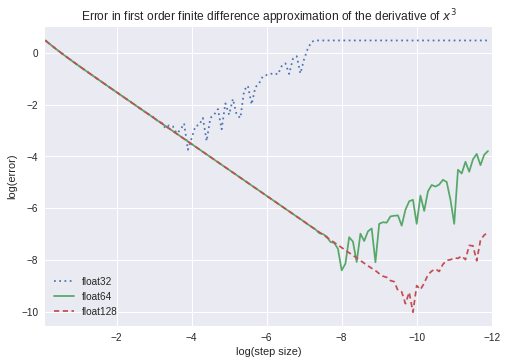
\includegraphics[width=\textwidth]{images/x^3_error_order1.png}
    \caption[Error in the approximation of the first derivative of $x^3$ by first order finite difference methods.]{This plot show error of using first order finite difference to approximate the derivative of $x^3$ vs the step size. Observe that the error falls almost linearly until the floating point errors start to dominate, after which it starts to grow erratically. Also, observe that for reasonable step sizes the error falls with a slope of 1, which is why such approximations are called to be of first order. }\label{fig:x^3_error_order1}
    \index{figures}
\end{figure}

In the beginning, irrespective of the float size, we have a straight line which turns into a wiggly mess as we keep on decreasing the step size. The reason for this sudden erratic increase in the error is floating point errors. One can clearly see that going form float32 to float64 is a big jump in accuracy. But in going to float128 from float64 the increase in the accuracy is not so dramatic, which is kind of expected as float128 has only 3 more significant digits over float64.

We can also use higher order methods, for example a second order method,

\begin{equation}
    y'(x_0)  \approx \frac{y(x_0 + h) - y(x_0 - h)}{2 \times h}
    \label{eq:d_second_order}
\end{equation}

To show that this a second order method one can taylor expand $y(x)$ around $x_0$ with step size $h$ and $-h$ and plug it back into the equation \ref{eq:d_second_order}. Figure \ref{fig:x^3_error_order2} shows the log(error) vs log(step size) graph for the second order approximation, notice that the slope of the line is now 2. Using higher order methods can give more accurate results for the same step size but they lead to other issues which we will briefly discuss later.

\begin{figure}[hbt!]
    \centering
    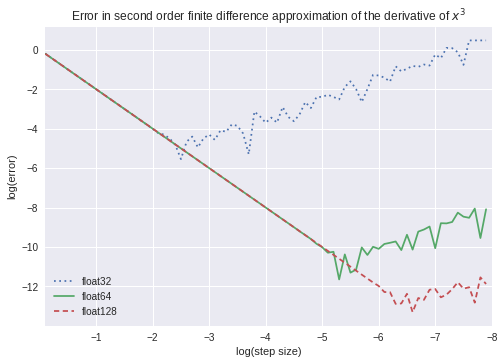
\includegraphics[width=\textwidth]{images/x^3_error_order2.png}
    \caption[Error in the approximation of the derivative of $x^3$ by second order finite difference methods.]{This plot show error of using second order finite difference to approximate the derivative of $x^3$ vs the step size. Observe that the error falls almost linearly until the floating point errors start to dominate, after which it starts to grow erratically. Also, observe that for reasonable step sizes the error falls along a line with slope 2 which is to be expected of a second order approximation. }\label{fig:x^3_error_order2}
    \index{figures}
\end{figure}


To give some perspective, while solving the scalar collapse equations we are going to use step size of the order $10^{-5}$, thus using float32 is just out of the picture. Also, our spatial domain will be [0,2] which implies that there will be at least $10^{5}$ operations per element (we can not decrease spatial step size without decreasing the time step size at the same time, something we will explore more in the next sections). From the discussions in the section \ref{para:addition_errors} we know that there is an error associated with each operation, thus, even though individual errors may be small given the size of calculations we are interested in they can quickly add up and destroy our simulations.





Having discussed the effect of the step size on the error of finite difference method we now turn to another major source of error. While talking about the error in the equation \ref{eq:1d_1o_error} we conveniently ignored the dependence of the error on the second derivative $y''(x_0)$. One can ask what will happen if the second derivative is very larger?

This is the question that figures \ref{fig:1/x_1}, \ref{fig:1/x_0.1} and \ref{fig:1/x_0.01}  try to answer. We know that,

\begin{equation}
    \frac{d^n}{dx^n}\left(\frac{1}{x}\right) = (-1)^n \frac{n!}{x^{(n+1)}}
\end{equation}

Because, close to the origin the derivatives are themselves very larger the error in our finite difference approximation keeps on increasing with as we get closer to the origin. This can be seen in the figures \ref{fig:1/x_1}, \ref{fig:1/x_0.1}, \ref{fig:1/x_0.01}. Notice how we have to take smaller and smaller step size to get the same accuracy as we get closer to the origin.

The approximation at $x=0.01$ is so bad that even taking the step size to be $10^{-10}$ is not giving very accurate answer (Figure \ref{fig:1/x_0.01}).

\textbf{The crux of the matter is that finite difference methods struggle when the function is changing very rapidly}. Something we will see in the results of our simulations.


\begin{figure}[hbt!]
    \centering
    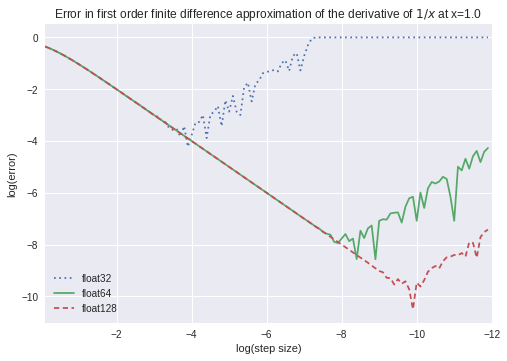
\includegraphics[width=0.8\textwidth]{images/1_x_error_at_1.png}
    \caption{This plot show error of using finite difference to approximate the derivative of $\frac{1}{x}$ vs the step size at $x = 1$.}
    \label{fig:1/x_1}
    \index{figures}
\end{figure}

\begin{figure}[hbt!]
    \centering
    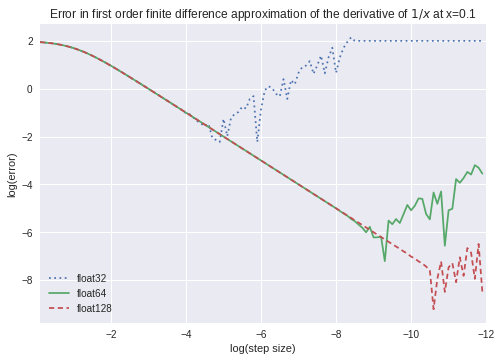
\includegraphics[width=0.8\textwidth]{images/1_x_error_at_p1.png}
    \caption{This plot show error of using finite difference to approximate the derivative of $\frac{1}{x}$ vs the step size at $x = 0.1$.}
    \label{fig:1/x_0.1}
    \index{figures}
\end{figure}


\begin{figure}[hbt!]
    \centering
    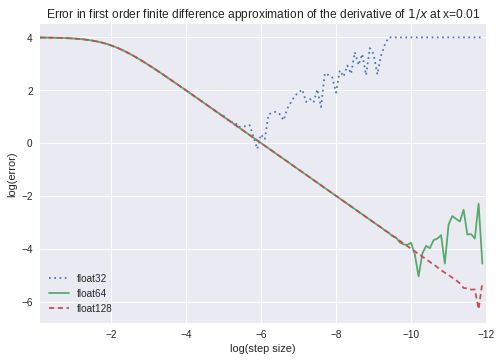
\includegraphics[width=0.8\textwidth]{images/1_x_error_at_p01.png}
    \caption{This plot show error of using finite difference to approximate the derivative of $\frac{1}{x}$ vs the step size at $x = 0.01$.}
    \label{fig:1/x_0.01}
    \index{figures}
\end{figure}


Although, this situation is still salvageable by using higher order methods as shown in the Figure \ref{fig:1/x_error_vs_order}. Notice that for the same step size the higher order methods are much more accurate, just by going to second order methods we are able to reduce the errors by a lot. Furthermore, using even higher order methods gives us a diminishing return which is one of the reasons why we will be using second order methods.

\begin{figure}[hbt!]
    \centering
    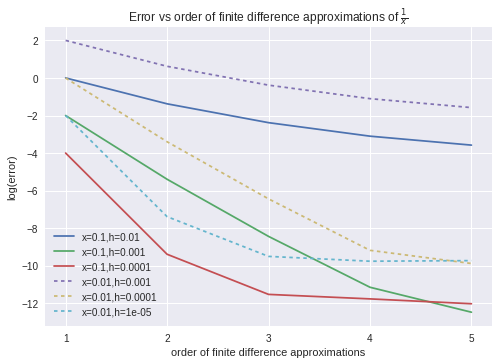
\includegraphics[width=\textwidth]{images/1_x_error_vs_order.png}
    \caption{This plot show error of using finite difference to approximate the derivative of $\frac{1}{x}$ vs the order of the approximation.}
    \label{fig:1/x_error_vs_order}
    \index{figures}
\end{figure}

% \Needspace{5\baselineskip}

\section{Solving scalar collapse equations}

Now that we have some understanding of how finite difference can be used to approximate derivatives, the next logical step is use it all to solve the differential equations that we have. In particular we want to solve,

\begin{equation}
    -r_{, t t}+r_{, x x}-e^{-2 \sigma} \cdot \frac{2 m}{r^{2}}=0
    \label{eqn:r_chap3}
\end{equation}

\begin{equation}
    -\psi_{, t t}+\psi_{, x x}+\frac{2}{r}\left(-r_{, t} \psi_{, t}+r_{, x} \psi_{, x}\right)=0
    \label{eqn:psi_chap3}
\end{equation}

\begin{equation}
    -\sigma_{, t t}+\sigma_{, x x}-e^{-2 \sigma} \cdot \frac{2 m}{r^{3}}+4 \pi\left(\psi_{, t}^{2}-\psi_{, x}^{2}\right)=0
    \label{eqn:sigma_chap3}
\end{equation}

\begin{equation}
    m_{, t}=4 \pi r^{2} \cdot e^{2 \sigma}\left[-\frac{1}{2} r_{, t}\left(\psi_{, t}^{2}+\psi_{, x}^{2}\right)+r_{, x} \psi_{, t} \psi_{, x}\right]
    \label{eqn:m_chap3}
\end{equation}

There are two parts to solving the scalar collapse equations:
\begin{enumerate}
    \item Solve the initial condition problem
    \item Evolve the initial configuration in time
\end{enumerate}

In general, solving initial conditions in GR is a very hard thing because we have to deal with elliptical partial differential equations. But in this case we are lucky as we are working in 1D and just need to solve a set of ordinary differential equations, which are much much easier and cheaper to solve.

We will be using finite difference methods to solve the initial conditions and then evolve the system in time, to do that we will first define some terminology and discretize the time-space domain. \index{Discretization} Discretization of the \index{time-space domain}time-space domain is shown in the figure \ref{fig:grid}, we will use uniform discretization which means that all time ($\Delta t$) and space ($\Delta x$) step sizes will be the same throughout the grid.



\begin{figure}[hbt!]
    \centering
    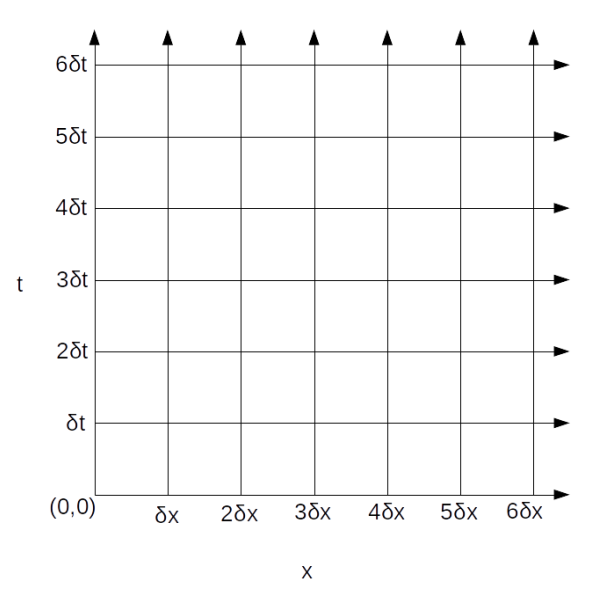
\includegraphics[width=\textwidth]{images/grid.png}
    \caption{Uniform discretization of time-space into a grid with space step size $\delta x$ and time step size $\delta t$.}
    \label{fig:grid}
    \index{figures}
\end{figure}

Furthermore, we will denotes the value of a variable $X(t,x)$ on the grid by,

\begin{equation}
    X^{n}_{j}  = X(n \delta t, j \delta x)
\end{equation}

Finite difference approximation of the derivatives $X^n_{j,x}$ and $X^n_{j,t}$ can be written as, (we will stop stop using $\approx$ sign from now on, but it should be clear from the context that we are talking about an approximation)

\begin{equation}
    X^n_{j,t} = \frac{X^{n+1}_{j} - X^{n-1}_{j}}{2 \delta t}
\end{equation}
\begin{equation}
    X^n_{j,x} = \frac{X^n_{j+1} - X^n_{j-1}}{2 \delta x}
\end{equation}

Similarly, second derivatives can be written as,


\begin{equation}
    X^n_{j,tt} = \frac{X^{n+1}_{j} -2X^n_j + X^{n-1}_{j}}{\delta t^2}
\end{equation}
\begin{equation}
    X^n_{j,xx} = \frac{X^n_{j+1} -2 X^n_j+ X^n_{j-1}}{\delta x^2}
\end{equation}




\subsection{Solving initial conditions}

From the section \ref{chap2:boundary_and_initial_conditions} we know the equations that we need to solve,


\begin{equation}
    r_{, x x}=e^{-2 \sigma} \cdot \frac{2 m}{r^{2}}
    \label{eqn:r_ic}
\end{equation}


\begin{equation}
    \sigma_{, x}= -2 \pi \cdot  \frac{\psi_{, x}^{2} \cdot r}{r_{,x}}- e^{-2 \sigma} \cdot \frac{ m}{r^{2}r_{, x}}
    \label{eqn:sigma_ic}
\end{equation}

\begin{equation}
    m_{, x}=4 \pi r^{2} \cdot e^{2 \sigma}\left[\frac{1}{2} r_{, x} \cdot \psi_{, x}^{2} \right]
    \label{eqn:m_ic}
\end{equation}


and their corresponding boundary conditions,

\begin{eqnarray}
    r(0 ,0) = 0 \implies r^0_0 = 0 \\
    r_{,x}(0 ,0) = 1 \implies r^0_{0,x} = 1 \\
    \sigma(0 ,0) = 1 \implies \sigma^0_0 = 0 \\
    m(0 ,0) = 1 \implies m^0_0 = 0
\end{eqnarray}

We used fourth order \index{Runge-Kutta}Runge-Kutta (RK4) method to solve these equations. RK4 method is the industry standard method to solve ordinary differential equations, RK4 is a fourth order method. Like most of the other finite difference methods RK4 is derived by solving a bunch of linear equations which we get by using taylor expansions. Its derivation can be found in any numerical analysis book and we will skip it because it will not add a lot to the current discussion.

Unlike partial differential equations, solving ordinary differential equations is mostly a "solved" problem in the sense that are plethora of robust packages that can solve a system of differential equations without any significant input from the user.

The standard way to solve a system of ordinary differential equations which condition higher order derivatives is to define new variables and get a set of first order ODEs. In our case we define a new variable $\bar r = r_{,x}$ which gives us,


\begin{equation}
    r_{,x} = \bar r
    \label{eqn:r2_ic}
\end{equation}

\begin{equation}
    \bar r_{,x}=e^{-2 \sigma} \cdot \frac{2 m}{r^{2}}
    \label{eqn:br2_ic}
\end{equation}


\begin{equation}
    \sigma_{, x}= -2 \pi \cdot  \frac{\psi_{, x}^{2} \cdot r}{\bar r}- e^{-2 \sigma} \cdot \frac{ m}{r^{2}\bar r}
    \label{eqn:sigma2_ic}
\end{equation}

\begin{equation}
    m_{, x}=4 \pi r^{2} \cdot e^{2 \sigma}\left[\frac{1}{2} \bar r \cdot \psi_{, x}^{2} \right]
    \label{eqn:m2_ic}
\end{equation}

Observe that there are no unknown derivatives in the RHS of these equations ($\psi _{,x}$ is known because we have the initial profile of $\psi$). At this point one can plug these equations in any differential equations solver, in our case we used DifferentialEquations.jl library for Julia language with tolerance set to $10^{-8}$.



\subsection{Time evolution}

For time evolution we will use second order \index{discretization}discretization of both the first and the second order derivatives. We will just show the discretization of the equation \ref{eqn:psi_discretized} which requires most work, rest of the equations can be discretized using the exact same procedure.

We should mention that to make things simple it is important that we solve the equation \ref{eqn:r_chap3} first followed by equation \ref{eqn:psi_chap3} after which other two equations can be solved in any order. The reason for this choice will become clear as we discretized the system.

\begin{equation}
    -\psi_{, t t}+\psi_{, x x}+\frac{2}{r}\left(-r_{, t} \psi_{, t}+r_{, x} \psi_{, x}\right)=0
    \label{eqn:psi_discretized}
\end{equation}

Writing the equation \ref{eqn:psi_discretized} in the notation we defined earlier we get:

\begin{equation}
    -\psi^n_{j, t t}+\psi^n_{j, x x}+\frac{2}{r^n_j}\left(-r^n_{j, t} \psi^n_{j, t}+r^n_{j, x} \psi^n_{j, x}\right)=0
    \label{eqn:psi_discretized_notation}
\end{equation}

Now we will use the second order finite difference approximations already discussed,

\begin{eqnarray}
    \label{eqn:beg_discretizations}
    \psi^n_{j,tt} &=& \frac{\psi^{n+1}_j - 2 \psi^{n}_j + \psi^{n-1}_j}{\delta t^2} \\
    \psi^n_{j,t} &=& \frac{\psi^{n+1}_j -  \psi^{n-1}_j}{2\delta t} \\
    \psi^n_{j,xx} &=& \frac{\psi^{n}_{j+1} - 2 \psi^{n}_j + \psi^{n}_{j-1}}{\delta x^2} \\
    \psi^n_{j,x} &=& \frac{\psi^{n}_{j+1} -  \psi^{n}_{j-1}}{2\delta x}
    \label{eqn:end_discretizations}
\end{eqnarray}

Other variables can be discretized in the same manner. Now we will make another simplifying assumption $\delta t = \delta x$, we use this assumption to make the equations look a little simpler and it does not affect the results. But, this is not something that can always be done, there are systems where making this assumption will lead to \index{superfluous oscillations} superfluous oscillations and \index{instability}instability. To prevent such instabilities we need to ensure that the temporal step size ($\delta t$) is bounded above by the spatial step size ($\delta x$) as dictated by the \index{Courant–Friedrichs–Lewy}Courant–Friedrichs–Lewy or \index{CFL}CFL conditions. Here it is enough to know that for our system we can take $\delta t = \delta x$ without causing instabilities.


Now, putting equations \ref{eqn:beg_discretizations}-\ref{eqn:end_discretizations} and similar equations for $r$ in the equation \ref{eqn:psi_discretized_notation} and cancelling out all the $\delta t$ and $\delta x$ we get,

\begin{multline}
    \psi^{n+1}_{j} + \psi^{n-1}_{j} - \psi^{n}_{j+1} - \psi^{n}_{j-1} = \frac{((\psi^{n}_{j+1} - \psi^{n}_{j-1})(r^{n}_{j+1} - r^{n}_{j-1}) - (\psi^{n+1}_{j} - \psi^{n-1}_{j})(r^{n+1}_{j} - r^{n-1}_{j}))}{2 r^n_j}
    \label{eqn:pis_discretized_long}
\end{multline}

What we need to do now is to collect all the $\psi^{n+1}_j$ terms on the LHS and rest of the equation on the RHS. This will give us the value of $\psi$ at the future time $(n+1) \delta t$ using the value of r and $\psi$ at the current time $n \delta t$ and the last time step $ (n-1) \delta t$.


One can see that this will lead to a very convoluted and hard to debug equation, there is actually a lot of simplification one can do by calculating few things in advance. First, notice that we can calculate all the spatial derivatives in advance because they only depend on the current time step ($n \delta t$). Furthermore, because we solved the equation \ref{eqn:r_chap3} before the current equation of $\psi$ we can also calculate and store the value of $r^n_{j,t}$ in advance. Using all this we can rewrite the equation \ref{eqn:pis_discretized_long} as,


\begin{multline}
    \psi^{n+1}_{j} + \psi^{n-1}_{j} - \psi^{n}_{j+1} - \psi^{n}_{j-1} = \frac{(4\delta t^2 (\psi^{n}_{j,x} \, r^{n}_{j,x}) - 2 \delta t(\psi^{n+1}_{j} - \psi^{n-1}_{j})\,r^{n}_{j,t})}{2 r^n_j}
    \label{eqn:final_psi}
\end{multline}

Now our equation is much more tangible and we can bring all the $\psi^{n+1}_j$ factors to the RHS and get the \index{time stepping equation}time stepping equation for $\psi$. We should explicitly mention that this is just a cosmetic change and the final answer will be the same up to floating point errors.

For other equations, the procedure is exactly the same with the only difference being that there will be no future time step term like $\psi^{n+1}_j$ in the LHS, which will make the corresponding time stepping equations much simpler.


\begin{figure}[hbt!]
    \centering
    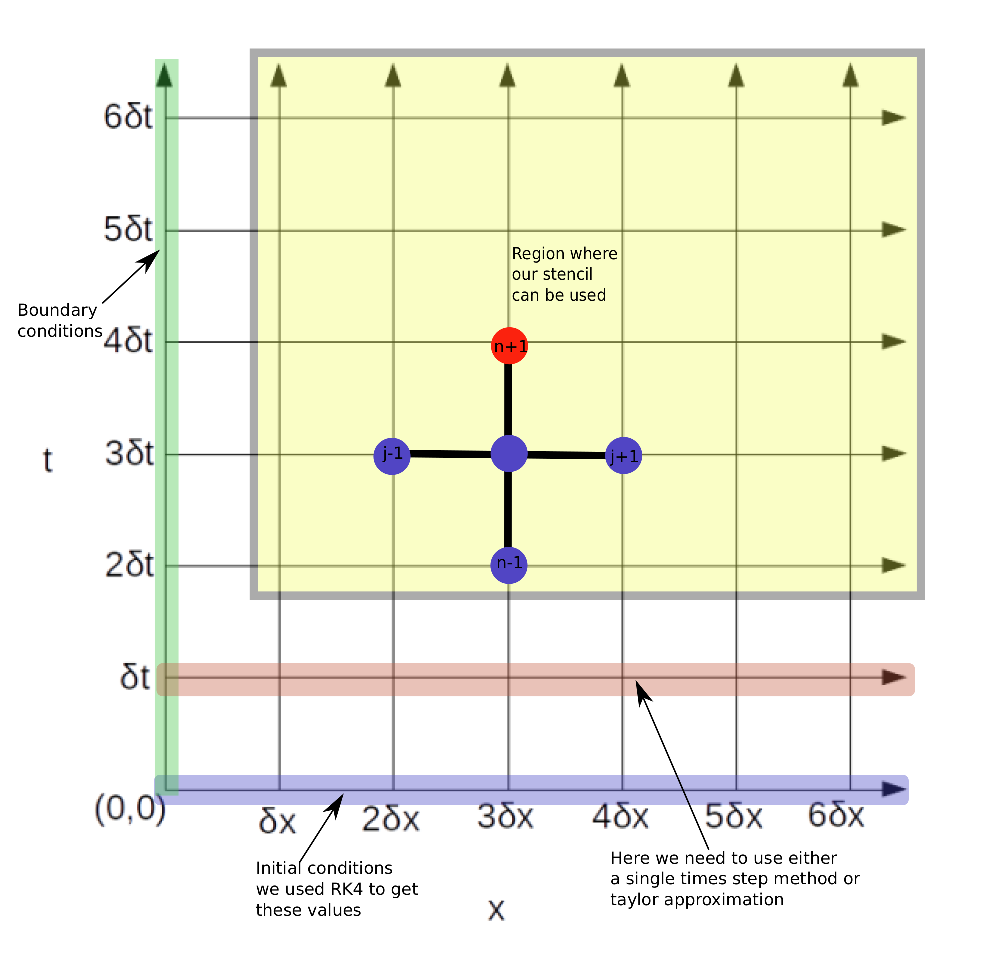
\includegraphics[width=\textwidth]{images/labelled_grid.eps}
    \caption[Stencil used and the computational grid]{This figure shows our computational domain and the stencil used. To calculate the value at any point on the grid we need the red dot of the stencil to be at that grid point, observe that we can not put the red circle of the stencil in the regions that are green, red and blue. \textbf{Yellow}: We can use our stencil in this region. \textbf{Red}: We have to use any other methods or stencils that only depend on the last time step, we used taylor series because it was the easiest to use in our case. \textbf{Blue}: This is the initial configuration of system that we evolve in time, i.e. initial conditions of our system.}
    \label{fig:grid_with_stencil_and_regions}
    \index{figures}
\end{figure}



There is one last technicality that we have to deal with before we can wrap up this section, we can not use the time stepping equation we derived above for the first time step ($n=1$). One can see this by plugging in $n=0$ in the equation \ref{eqn:final_psi}, which is supposed to give the value of $\psi$ at time $\delta t$. But, doing so will lead to a term of type $\psi^{-1}_j$ which is of course not something we can deal with using our current \index{stencil}stencil (time stepping equations).


This brings us to one of the reason why higher order methods are in general harder to code and reason about. Our finite difference approximation uses three space and and last two time steps thus, we can not use it at the boundaries or for the first time step. Figure \ref{fig:grid_with_stencil_and_regions} shows various regions where we can not use out time stepping equations. This becomes a much bigger issue if one uses even higher order finite difference methods as they will use more than 3 spatial points per calculation.


\subsection{Dealing with the first time step}

To calculate the value of the variables at time $t = \delta t$ we used taylor series, again for brevity we will show the procedure just for $\psi$.

\begin{equation*}
    \psi(\delta t,x) = \psi(0,x) + \delta t\, \psi_{,t}(0,x) + \frac{\delta t^2}{2} \, \psi_{,tt}(0,x) + O(\delta t^3)
\end{equation*}


First notice that we are using taylor series up to $O(\delta t^3)$, this is essential because our time stepping equations are of second order. If we do not use higher order taylor series then the first order error will propagate to later time steps defeating the purpose of using second order stencil. This should be kept in mind while using single step methods as well, because they are not as accurate as our second order method for the same step size. In that case we need to divide the time step $\delta t$ into smaller time steps and take multiple small time steps via a single step stencil to get to the first time step ($\delta t$).


Another convenience in using taylor series in our case is that $X_{,t}(0,x) = 0$ for $X = \psi, r ,\sigma$ because of our boundary conditions. Thus we only need to solve,

\begin{equation*}
    \psi(\delta t,x) = \psi(0,x) + \frac{\delta t^2}{2} \, \psi_{,tt}(0,x) + O(\delta t^3)
\end{equation*}

$X_{,tt}(0,x)$ can be easily obtained using the equations \ref{eqn:r_chap3}-\ref{eqn:sigma_chap3}.


For $m$ we need to do some work, first we have to take time derivative of the equation \ref{eqn:m_chap3} and then use it in the taylor series.


\subsection{Boundary conditions}
\label{chap3:boundary_conditinos}

Boundary conditions (refer section \ref{chap2:boundary_and_initial_conditions}) at $x=0$ are easy to implement, for example, $r_t(t,0) = 0$ when discretized is same as $r^{n}_0 = r^{n-1}_0$. Similarly, $\psi_{,x}(t,0) = 0 $ when discretized implies $\psi^{n}_0 = \psi^{n}_1$.

Now, we need the boundary conditions at the outer boundary, in the physical space this is same as the boundary conditions at infinity. But we are working with a finite domain so we need some kind of boundary conditions at the spatial edge of our computational domain. There are multiple ways to deal with this, one is to simply use \index{extrapolation boundary conditions}extrapolation boundary conditions. Another is to use absorbing boundary conditions or free boundary conditions, both of these are usually more accurate but at the same time harder to implement.

In our case we are lucky because we have a system of hyperbolic equations and in addition to that we do not need to evolve the system for longer periods.
As it turns out for hyperbolic systems there is a natural light cone kind of domain associated with each grid point and it can only be affected by the grid points in that cone.
This can be intuitively seen in the Figure \ref{fig:grid_outer_boundary_conditions}. Because of this property we can use extrapolation boundary conditions without it affecting our calculations.

\begin{figure}[hbt!]
    \centering
    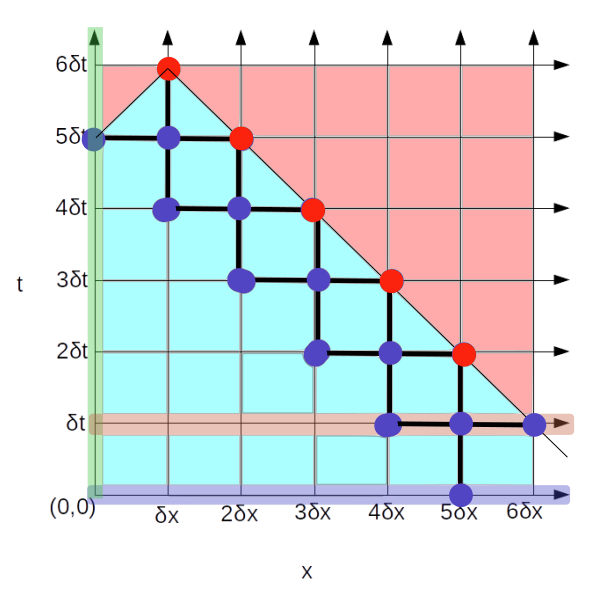
\includegraphics[width=\textwidth]{images/grid_outer_boundary_condition.png}
    \caption{This figure shows the grid points that can affect the grid point X at $(6 \,\delta t, \delta x)$. Grid points in blue can affect the grid point X while grid points in red can not.}
    \label{fig:grid_outer_boundary_conditions}
    \index{figures}
\end{figure}


\section{How do we check the accuracy of the numerical results?}

Because we do not have an analytical solution to compare with, we need some others ways to get confidence in our results. We used two commonly used methods to check the reliability of our numerical results,

\begin{enumerate}
    \item Using constraint equations
    \item Showing that the results are independent of the step size
\end{enumerate}

\subsection{Using constraint equations}

As mentioned in the last chapter we get two constraint equations along with the three evolution equations. We can use these constraint equations to check whether our results are correct or not. This is the primary method we used and there will be more discussion about the values of constraints in the next chapter.


\subsection{Showing that the results are independent of the step size}

We have developed the whole algorithm but there is still the question of what step size should we use. If the step size is too small then our equations will not be a good approximation of the original equations. On the other hand if the step size is too small then it may take a lot of time to evolve the system. The standard way of choosing a step size is to decide on a tolerance and try out several step sizes. As we keep on decreasing the step size there will be a threshold after which the answers will effectively become independent of the step size up to the tolerance. We can then choose any step size smaller than that threshold.

This also acts as a check for the algorithm because any dependence of the answer on the step sizes smaller than the threshold is a clear indication that our algorithms are not true representation of the underlying differential equations.
This method of checking the finite difference may fail for chaotic systems, but we are not dealing with those here.

Then there are obvious problem specific sanity checks like there are no superfluous oscillations. We can also check for extreme cases, for example, in our system if we take the initial configuration of the scalar field to be uniformly zero then we do not expect to see any kind of evolution.






This sums up our numerical part, in the next chapter we will discuss about the profiles of $\psi$ used and the results.